\documentclass[a4paper, twoside]{report}

%%%%%%%%%%%%%%%%%%%%%%%%%%%%%%%%%%%%%%%
%%%%%%%%%%%%% IMPORT PACKAGES %%%%%%%%%
%%%%%%%%%%%%%%%%%%%%%%%%%%%%%%%%%%%%%%%
\usepackage[hidelinks]{hyperref}
\usepackage{subfigure}
\usepackage{fancyvrb}
\usepackage{amsmath, amsfonts, amsthm, amssymb}
\usepackage{stmaryrd}
\usepackage{verbatim}
\usepackage{graphicx}
\usepackage{setspace}
\usepackage[ruled, vlined]{algorithm2e}
\graphicspath{{Figures/}}

%%%%%%%%%%%%%%%%%%%%%%%%%%%%%%%%%%%%%%%5
\usepackage{listings}
\usepackage{xcolor}
\definecolor{codegreen}{rgb}{0,0.6,0}
\definecolor{codegray}{rgb}{0.5,0.5,0.5}
\definecolor{codepurple}{rgb}{0.58,0,0.82}
\definecolor{backcolour}{rgb}{0.95,0.95,0.92}

\lstdefinestyle{mystyle}{
    backgroundcolor=\color{backcolour},   
    commentstyle=\color{codegreen},
    keywordstyle=\color{magenta},
    numberstyle=\tiny\color{codegray},
    stringstyle=\color{codepurple},
    basicstyle=\ttfamily\footnotesize,
    breakatwhitespace=false,         
    breaklines=true,                 
    captionpos=b,                    
    keepspaces=true,                 
    numbers=left,                    
    numbersep=5pt,                  
    showspaces=false,                
    showstringspaces=false,
    showtabs=false,                  
    tabsize=2
}
\lstset{style=mystyle}
%%%%%%%%%%%%%%%%%%%%%%%%%%%%%%%%%%%%%%%%
%%%%%%%%%%%%%%%%%%%%%%%%%
\newtheorem{theorem}{Theorem}[section]
\newtheorem{exa}{Example}[section]
\newtheorem{corollary}[theorem]{Corollary}
\newtheorem{lemma}[theorem]{Lemma}
\newtheorem{proposition}[theorem]{Proposition}

\theoremstyle{definition}
\newtheorem{definition}[theorem]{Definition}
\newtheorem{remark}[theorem]{Remark}
\newtheorem{notation}[theorem]{Notation}
\newtheorem{assumption}[theorem]{Assumption}
\newtheorem{conjecture}[theorem]{Conjecture}

\newcommand{\ind}{1\hspace{-2.1mm}{1}} %Indicator Function
\newcommand{\I}{\mathtt{i}}
\newcommand{\D}{\mathrm{d}}
\newcommand{\E}{\mathrm{e}}
\newcommand{\RR}{\mathbb{R}}
\newcommand{\sgn}{\mathrm{sgn}}
\newcommand{\atanh}{\mathrm{arctanh}}
\def\equalDistrib{\,{\buildrel \Delta \over =}\,}
\numberwithin{equation}{section}


%%%%%%%%%%%%%%%%%%%%%%%%%%%%%%%%%%%%%%%%%%%%%%%
%%%%%%%%%%%%%%%%%%%%%%%%%%%%%%%%%%%%%%%%%%%%%%%
%% Sets page size and margins
\usepackage[a4paper,top=3cm,bottom=2cm,left=3cm,right=3cm,marginparwidth=1.75cm]{geometry}
\title{Solving the Collatz conjecture}
\author{Jack JACQUIER (CID: 00000000)}

\begin{document}
\begin{titlepage}

\newcommand{\HRule}{\rule{\linewidth}{0.5mm}} 

\includegraphics[width=8cm]{logo.png}\\[1cm]
\center

\quad\\[1.5cm]
\textsc{\Large Imperial College London}\\[0.5cm]
\textsc{\large Department of Mathematics}\\[0.5cm]

\makeatletter
\HRule \\[0.2cm]
\begin{spacing}{2.5}
{\huge \bfseries \@title}
\end{spacing}
\HRule \\[1.5cm]
 
\begin{minipage}{0.8\textwidth}
\begin{flushleft} \large
\emph{Author:}
\@author
\end{flushleft}
\end{minipage}
~\vspace{2cm}
\makeatother


{\large A thesis submitted for the degree of}\\[0.5cm]
{\large \emph{MSc in Mathematics and Finance, 2022-2023}}\\[0.5cm]

\vfill

\end{titlepage}

\mbox{}\newline\vspace{10mm} \mbox{}\LARGE
%
{\bf Declaration} \normalsize \vspace{5mm}

The work contained in this thesis is my own work unless otherwise stated.

\newpage

\renewcommand{\abstractname}{Acknowledgements}
\begin{abstract}
  This is where you usually thank people who have provided useful assistance, feedback,...., during your project.
\end{abstract}

\newpage

\renewcommand{\abstractname}{Abstract}
\begin{abstract}
  The abstract is a short summary of the thesis' contents.
  It should be about half a page long and be accessible by someone not familiar with the project.
  The goal of the abstract is also to tease the reader and make him want to read the whole thesis.
\end{abstract}

\tableofcontents
\listoffigures
\listoftables

%%%%%%%%%%%%%%%%%%%%%%%%%%%%%%%%%%%%%%%%%%%%%%%
\chapter*{Introduction}

The introduction is one of the most important components of the thesis.
It should be readable by anyone,
including people without prior knowledge of the field.
It should progressively introduce the main topic of the paper, and explain the structure of the thesis.
In Section~\ref{sec:HowTo}, we shall provide several examples of clearly written examples,
whereas Section~\ref{sec:WhatNotToDo} will gather a certain number of common mistakes and errors.

%%%%%%%%%%%%%%%%%%%%%%%%%%%%%%%%%%%%%%%%%%%%%%%
\begin{remark}
  Please bear in mind the following when writing your thesis (or anything for that matter):
  you are not writing for you. You are writing for an audience, who will (have to) read your work.
  Please be considerate, and explain everything clearly.
  In this case, the audience could be your fellow MSc students,
  with some general knowledge of the area, but maybe not specialised to your particular topic.
\end{remark}


\newpage
%%%%%%%%%%%%%%%%%%%%%%%%%%%%%%%%%%%%%%%%%%%%%
\chapter{How to write mathematics}\label{sec:HowTo}
In this section, we show some examples of properly written mathematical expressions and sentences.
In the header of your thesis, you can define \LaTeX \ shortcuts to write more quickly.



%%%%%%%%%%%%%%%%%%%%%%%%%%%%%%%%%%%%%%%%%%
\section{The Black-Scholes model}
Consider a given probability space $(\Omega, \mathcal{F},\mathbb{P})$
supporting a Brownian motion~$(W_t)_{t\geq 0}$.
In the Black-Scholes model, the stock price process~$(S_t)_{t\geq 0}$ is the unique strong solution to
the following stochastic differential equation:
\begin{equation}\label{eq:BS}
  \frac{\D S_t}{S_t} = r \D t + \sigma \D W_t,
  \qquad S_0>0,
\end{equation}
where $r\geq 0$ denotes the instantaneous risk-free interest rate and $\sigma>0$ the instantaneous volatility.
A European call price $C_t(S_0,K,\sigma)$ with maturity $t>0$ and strike $K>0$
pays at maturity $(S_t-K)_+=\max(S_t-K,0)$.
When the stock price follows the Black-Scholes SDE~\eqref{eq:BS},
Black and Scholes~\cite{black1973pricing} proved that its price at inception is worth
$$
  C_t(S_0,K,\sigma) = S_0\mathcal{N}(d_+) - K\E^{-rt}\mathcal{N}(d_-),
$$
where
$$
  d_{\pm} := \frac{\log\left(S_0 \E^{rt}/K\right)}{\sigma\sqrt{t}} \pm \frac{\sigma\sqrt{t}}{2},
$$
and where~$\mathcal{N}$ denotes the cumulative distribution function of the Gaussian random variable.




%%%%%%%%%%%%%%%%%%%%%%%%%%%%%%%%%%%%%%%%%%%%%%%
%%%%%%%%%%%%%%%%%%%%%%%%%%%%%%%%%%%%%%%%%%%%%%%




%%%%%%%%%%%%%%%%%%%%%%%%%%%%%%%%%%%%%%%%%%
\subsection{More complicated mathematical expressions}
In the Heston model, the stock price is the unique strong solution to the following stochastic differential equation:
\begin{equation}\label{eq:Heston}
  \begin{array}{rll}
    \D S_t                   & = S_t \sqrt{V_t} \D W_t,                        & S_0 = s>0,   \\
    \D V_t                   & = \kappa(\theta-V_t)\D t + \xi\sqrt{V_t}\D Z_t, & V_0 = v_0>0, \\
    \D \langle W, Z\rangle_t & = \rho \D t,
  \end{array}
\end{equation}
where $\kappa, \xi, \theta, v_0, s>0$ and the correlation parameter $\rho$ lies in $[-1,1]$.
In the system~\eqref{eq:Heston}, the process $(V_t)_{t\geq 0}$ represents the instantaneous
variance (squared volatility) of the underlying stock price~$S$.
Existence of a unique strong solution for the variance process (also called the Feller process)
are guaranteed by the Yamada-Watanabe conditions~\cite[Proposition 2.13, page 291]{karatzas1991brownian}).


%%%%%%%%%%%%%%%%%%%%%%%%%%%%%%%%%%%%%%%%%%
\subsection{Writing Definitions, Theorems,...}
All the environments for Definitions, Theorems,... are already defined in \LaTeX.
Here is an example:
\begin{theorem}[Static replication]\label{thm:StaticReplication}
  Let~$f:\RR\to\RR$ be a $\mathcal{C}^2$ function, and $F$ a non-negative constant.
  A European option with payoff $f(S)$ can be fully statically replicated using only cash,
  the underlying stock and a continuum of European Calls and Puts.
\end{theorem}
\begin{proof}
  By the fundamental theorem of calculus, we have
  \begin{align*}
    f(S) & = f(F) + \ind_{\{S>F\}}\int_F^S f'(u)\D u  \ - \  \ind_{\{S<F\}}\int_S^F f'(u)\D u                                       \\
         & = f(F) + \ind_{\{S>F\}}\int_F^S\left[f'(F) + \int_F^u f''(v)\D v\right]\D u
    - \ind_{\{S<F\}}\int_S^F \left[f'(F) - \int_u^F f''(v) \D v\right]\D u                                                          \\
         & = f(F) + f'(F) (S-F) + \ind_{\{S>F\}}\int_F^S \int_v^S f''(v)\D u \D v  + \ind_{\{S<F\}}\int_S^F \int_S^v f''(v)\D v\D u \\
         & = f(F) + f'(F) (S-F) + \ind_{\{S>F\}}\int_F^S f''(v)(S-v) \D v  + \ind_{\{S<F\}}\int_S^F f''(v) (v-S)\D v                \\
         & = f(F) + f'(F) (S-F) + \ind_{\{S>F\}}\int_F^\infty f''(v)(S-v)_+ \D v  + \ind_{\{S<F\}}\int_0^F f''(v) (v-S)_+ \D v
  \end{align*}
\end{proof}



%%%%%%%%%%%%%%%%%%%%%%%%%%%%%%%%%%%%%%%%%%%%%%%%%%%%
\subsection{Further examples}
Here is an example of a matrix in $A\in\mathcal{M}_n(\RR)$:
$$
  A =
  \begin{pmatrix}
    a_{11} & a_{12} & \ldots & a_{1n}  \\
    a_{21} & \ddots & \ddots & \vdots  \\
    \vdots & \ddots & \ddots & \vdots  \\
    a_{n1} & \ldots & \ldots & a_{1n}.
  \end{pmatrix}
$$

%%%%%%%%%%%%%%%%%%%%%%%%%%%%%%%%%%%%%%%%%%%%%%%%%%%%
%%%%%%%%%%%%%%%%%%%%%%%%%%%%%%%%%%%%%%%%%%%%%%%%%%%%
\subsection{Citing other papers}
When quoting a book, paper,..., please indicate the \textbf{precise} (page, which theorem, chapter, section,...) reference,
for example~\cite[Proposition 2.13, page 291]{karatzas1991brownian}), instead of just~\cite{karatzas1991brownian}.

You can also reference papers that have not been published yet, such as~\cite{mytnik2015uniqueness}.

The standard and easiest way to do so is as follows:
\begin{itemize}
  \item Go to \href{https://scholar.google.com/}{https://scholar.google.com/}
  \item Type the title of the paper/book/...
  \item Once you find the correct reference, click on \emph{Cite} below and open the \emph{BibTeX} link
  \item Copy-paste the whole output into your "biblio.bib" file
  \item All references will be automatically updated in the bilbiography.
\end{itemize}
%%%%%%%%%%%%%%%%%%%%%%%%%%%%%%%%%%%%%%%%%%%%%%%%%%%%
%%%%%%%%%%%%%%%%%%%%%%%%%%%%%%%%%%%%%%%%%%%%%%%%%%%%
\section{Common Errors}\label{sec:WhatNotToDo}
We list below some recommendations and common mistakes and errors.
The reader should check in the previous sections how these were used in a proper way.

\begin{itemize}
  \item When referencing an equation, use \texttt{eqref} instead of \texttt{ref}.
        However, when referencing a definition, theorem...., use \texttt{ref}
  \item Mathematical expressions are integral parts of the sentence,
        and therefore punctuation rules apply.
        They are therefore followed by commas, full stops, semicolons,... See examples above.
  \item Most mathematical functions are already built in \LaTeX,
        so that `ln' should be written $`\log'$:
        $$
          \log\left(x + \frac{\mathrm{atan}(x)}{y}\right)
          \qquad\text{instead of}\qquad
          ln\left(x + \frac{atan(x)}{y}\right).
        $$
        Note here, that the \texttt{atan} function is not already defined,
        so that we used \texttt{mathrm\{atan\}} instead, to be consistent.
        This obviously holds for $\exp$, $\cos$, $\tan$, $\min$, $\max$...
  \item Bibliography: papers should be referenced precisely, with the journal, volume, year, pages, publisher....
        If the paper is not published (yet), indicate the web link to find it (SSRN or arXiv).
        Also, at least in mathematics, authors are listed in alphabetical order.
  \item There is a difference between $x:=a$ and $x=a$.
        The former is a definition for~$x$, whereas in the latter, both~$x$ and~$a$ have already been defined,
        and this is a statement comparing them.
        It is usually a good idea to use $x:=a$ whenever you \textbf{define} some quantities.
  \item The following notation (even though often used) is wrong:
        $\sigma_t$ \textbf{IS NOT} a process; it is a random variable representing the (random) state
        of the process $\sigma=(\sigma_s)_{s\geq 0}$ at time~$s=t$.
        Likewise, $f(x)$ is not a function, whereas~$f$, or~$f(\cdot)$ is.
  \item Do not write `Thanks to \textrm{Python}'; maybe `Using \textrm{Python}' is preferable.
  \item Overfull lines must be avoided at all costs. For a long expression, one solution is, for example,
        to break it into smaller pieces.
        For example
        $$
          \mathcal{N}\left(d_+^*(\tau)\right)-\E^k\left(1-\mathcal{N}\left(-d_-^*(\tau)\right)\right)
          = 1- \frac{1}{\sqrt{2\pi}}\exp\left(-\frac{1}{2}d_{+}^*(\tau)^2\right)
          \left\{\frac{1}{d_{+}^*(\tau)} -\frac{1}{d_{-}^*(\tau)}
          + \frac{1}{d_{-}^*(\tau)^3} - \frac{1}{d_{+}^*(\tau)^3}
          + \mathcal{O}\left(\frac{1}{d_{+}^*(\tau)^5}\right)\right\},
        $$
        should be written, for example,
        \begin{align*}
          \mathcal{N}\left(d_+^*(\tau)\right)-\E^k\left(1-\mathcal{N}\left(-d_-^*(\tau)\right)\right)
          = & 1- \frac{1}{\sqrt{2\pi}}\exp\left(-\frac{1}{2}d_{+}^*(\tau)^2\right)
          \left\{\frac{1}{d_{+}^*(\tau)} -\frac{1}{d_{-}^*(\tau)}\right.           \\
            & \left.
          + \frac{1}{d_{-}^*(\tau)^3} - \frac{1}{d_{+}^*(\tau)^3}
          + \mathcal{O}\left(\frac{1}{d_{+}^*(\tau)^5}\right)\right\},
        \end{align*}
  \item Write Call and Put options instead of call and put options.
  \item Because `'i' / `e' ` `d' can be used both for complex argument / exponential / differential,
        and dummy variables, it is a good idea to use slightly different symbols, for instance:
        $$
          \int_{0}^{1}\sum_{i=1}^{n}\E^{\I i e^d} \D e.
        $$
        THe \LaTeX command is \texttt{mathrm\{e\}} and \texttt{mathrm\{i\}}.
  \item When using the indicator function, it is better to write
        $\ind_{\{x\in A\}}$ than $\ind_{(x\in A)}$ or $\ind_{x\in A}$
        since the first notation makes it clear that $\{x\in A\}$ is indeed an event.
  \item Try to avoid abbreviations: wlog, lhs, rhs....
  \item Do not use $\exists$, $\forall$ and other cryptic symbols.
        Words are more powerful and easier to read.
  \item Do not number all equations. Only those you need to quote.
\end{itemize}

%%%%%%%%%%%%%%%%%%%%%%%%%%%%%%%%%%%%%%%%%%%%5
\chapter{Inserting figures, codes, and Plagiarism issues}
%%%%%%%%%%%%%%%%%%%%%%%%%%%%%%%%%%%%%%%%%%
\section{Inserting a picture}
Here are some examples of how to insert pictures and how to refer to a particular one (see Figure~\ref{fig:Pict} for example).
Since you do not necessarily know where the figure will actually appear,
you should never refer to it with a sentence such as {\it "As shown here:"}


\begin{figure}[h!]
  \centering
  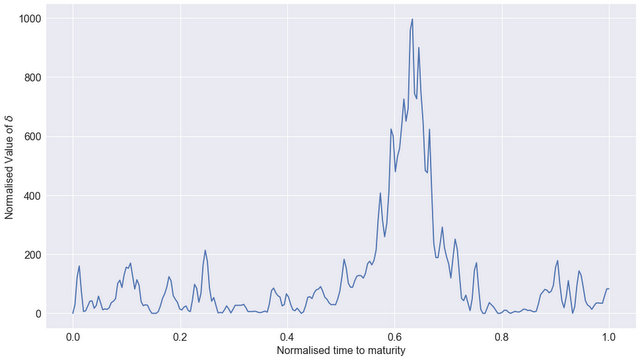
\includegraphics[scale=0.4]{profileNorm.jpg}
  \caption{This is the caption for the figure, detailing what the figure represents.}
  \label{fig:Pict}
\end{figure}


Some comments are in order:
\begin{itemize}
  \item It is often more convenient (as is done here) to gather all the pictures in a subfolder "Figures". The command \emph{graphicspath{{Figures/}}} in the preamble of the tex file tells \LaTeX where to look them up.
  \item Only insert a picture to illustrate something.
  \item A picture is not a proof, but a visual help.
  \item Make sure the picture is clear: axes readable, different plots easy to distinguish, fonts not too small....
  \item Use the \emph{.eps} format instead of \emph{.pdf}/\emph{.jpeg}/... (better quality).
\end{itemize}

%%%%%%%%%%%%%%%%%%%%%%%%%%%%%%%%%%%
\subsection{Nice plot vs bad plot}

Figure~\ref{fig:fig2} contains two plots of the same function.
Subfigure~\ref{fig:fig2sub1} shows a bad version while Subfigure~\ref{fig:fig2sub2}
shows a much clearer figure.
The problems with Subfigure~\ref{fig:fig2sub1} are the following:

\begin{figure}[htbp]
  \centering
  \subfigure[Bad figure.]{
    \label{fig:fig2sub1}
    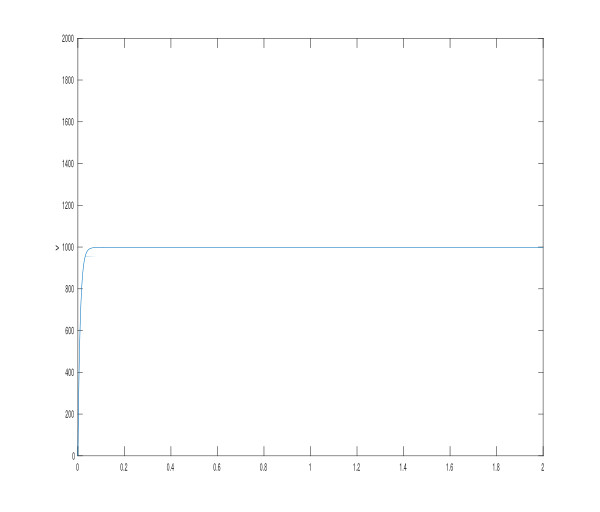
\includegraphics[scale=0.3]{figure1.jpg}}
  \subfigure[Goof figure.]{
    \label{fig:fig2sub2}
    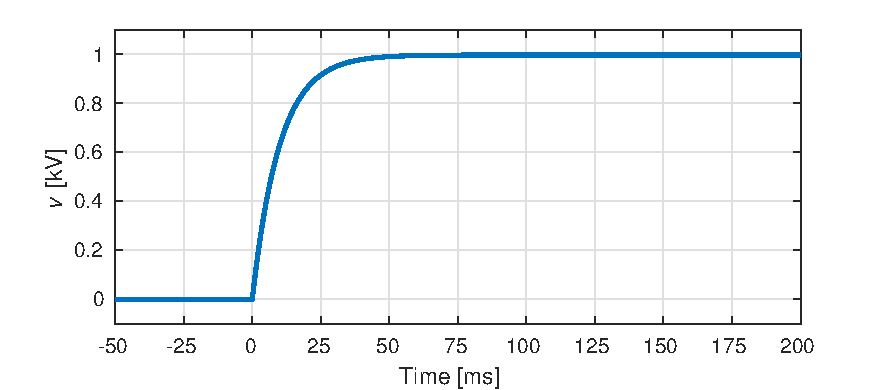
\includegraphics[scale=0.5]{figure2.pdf}}
  \caption{An image with two subfigures.}
  \label{fig:fig2}
\end{figure}

\begin{enumerate}
  \item The font size is too small to be read properly.
  \item The axes are not labeled properly: the horizontal axis does not have units. and the vertical one does not have labels.
  \item The left figure has too much blank space because the axes limits are wrongly chosen.
  \item The scaling of the figure did not preservethe original aspect ratio (in particular the font size).
  \item The width of the plot is too thin and scarcely visible.
  \item The figure was exported as a bitmap (png, jpg, bmp) instead of vector format (eps, svg, pdf).
\end{enumerate}


%%%%%%%%%%%%%%%%%%%%%%%%%%%%%%%%%%%%%%%%%%%%%%%%
%%%%%%%%%%%%%%%%%%%%%%%%%%%%%%%%%%%%%%%%%%%%%%%%

\section{Inserting a table}
You can of course include tables (and these will be listed in the List of Tables above):

\begin{table}[h!]
  \centering
  \begin{tabular}{|c|c|c|}
    \hline
    Simulation ID & $X$  & $Y$ \\
    \hline
    1             & 0.1  & 1.2 \\
    2             & -0.2 & 2.3 \\
    3             & 0.5  & 1.1 \\
    \hline
  \end{tabular}
  \caption{Caption for the table}
\end{table}
%%%%%%%%%%%%%%%%%%%%%%%%%%%%%%%%%%%%%%%%%%%%%%%%
%%%%%%%%%%%%%%%%%%%%%%%%%%%%%%%%%%%%%%%%%%%%%%%%

\section{Inserting code}
This section gathers a few DOs / DON'Ts regarding implementation.

\begin{itemize}
  \item Code has to be annotated. Otherwise, it is impossible (i) to read and, most importantly,
        (ii) to be used by someone else (remember that you will be working with other people).
  \item Code available on the Internet is not necessarily (actually scarcely) correct.
        If you use some, (i) be careful and check it, (ii) reference it precisely.
  \item Code should be usable. So all the variables should be input of the main functions.
        In order to change the values of one parameter and re-run the code, the user should not have to dive into the code.
  \item You do not necesssarily need to have all the code in your thesis, as reading code is not particularly pleasant. That said, it might be convenient to illustrate some points. If you do, here is a suggestion on how to do so, using the \emph{lstlisting} package (which you need to import in the preamble of your file:
        \begin{lstlisting}[language=python,numbers=none]
import matplotlib.pyplot as plt
import pandas as pd
from yahoo_fin import options
plt.style.use("seaborn")
TT = options.get_expiration_dates("goog")
chain = options.get_options_chain("goog")
chain["calls"].head()
\end{lstlisting}
\end{itemize}

%%%%%%%%%%%%%%%%%%%%%%%%%%%%%%%%%%%%%%%%%%%%%
%%%%%%%%%%%%%%%%%%%%%%%%%%%%%%%%%%%%%%%%%%%%%
\section{Adding references}


%%%%%%%%%%%%%%%%%%%%%%%%%%%%%%%%%%%%%%%%%%%%%
%%%%%%%%%%%%%%%%%%%%%%%%%%%%%%%%%%%%%%%%%%%%%
\section{Plagiarism}
Plagiarism is a fundamental issue, and should not be taken lightly.
According to Oxford Dictionary, it is
\textit{the practice of taking someone else's work or ideas and passing them off as one's own}.
For the thesis itself, plagiarism will be \textbf{severely sanctioned}, according to
\href{http://www.imperial.ac.uk/student-records-and-data/for-current-students/undergraduate-and-taught-postgraduate/exams-assessments-and-regulations/plagiarism-academic-integrity--exam-offences/}
{Imperial College's regulations}
for Imperial College's plagiarism framework.
According to \href{https://www.imperial.ac.uk/admin-services/library/research-support/plagiarism-awareness-for-researchers/supervising-plagiarism-by-students/}{College regulations},
the following are examples of plagiarism (see the previous links for precisions):
\begin{itemize}
  \item Collusion.
  \item Copy and paste.
  \item Word switch.
  \item Misinterpreting common knowledge.
  \item Concealing sources.
  \item Self plagiarism.
\end{itemize}

This obviously applies to any material you submit, whether report or code.

The easiest way to add a reference is as follows:
\begin{itemize}
  \item Go to \href{https://scholar.google.com/}{scholar.google.com/}
  \item Type in the title of the paper/book/...
  \item Find the item corresponding to the reference, and click on the \emph{Cite} link.
  \item Select the \emph{BibTeX} link
  \item Copy/paste the whole reference into your ".bib" file
  \item The ID of the reference (to be used in your ".tex" file) is the first part of the pasted text.
\end{itemize}
%%%%%%%%%%%%%%%%%%%%%%%%%%%%%%%%%%%%%%%%%%%%%%%
%%%%%%%%%%%%%%%%%%%%%%%%%%%%%%%%%%%%%%%%%%%%%%%



%%%%%%%%%%%%%%%%%%%%%%%%%%%%%%%%%%%%%%%%%%%%%%%

\newpage
\chapter*{Conclusion}
This is the conclusion, which summarises the main achievements of the thesis,
and may discuss quickly some open problems.


%%%%%%%%%%%%%%%%%%%%%%%%%%%%%%%%%%%%%%%%%%%%%%%
%%%%%%%%%%%%%%%%%%%%%%%%%%%%%%%%%%%%%%%%%%%%%%%
\newpage
\appendix
\chapter{Technical Proofs}
\section{Example of an Appendix}\label{app:Appendix}
This is Appendix~\ref{app:Appendix}, which usually contained supporting material,
or complicated proofs that might make the main text above less readable / fluid.

%%%%%%%%%%%%%%%%%%%%%%%%%%%%%%%%%%%%%%%%%%%%%%%
%%%%%%%%%%%%%%%%%%%%%%%%%%%%%%%%%%%%%%%%%%%%%%%
\bibliographystyle{unsrt}
\bibliography{biblio}
\addcontentsline{toc}{chapter}{Bibliography}

\end{document}